\documentclass[11pt,a4paper]{article}

\usepackage[utf8]{inputenc}
\usepackage[T1]{fontenc}
\usepackage[margin=2.5cm]{geometry}
\setlength{\headheight}{14pt}
\usepackage[colorlinks=true,linkcolor=red!60!black,urlcolor=blue!60!black,citecolor=blue!60!black]{hyperref}
\usepackage{xcolor}
\usepackage{booktabs}
\usepackage{listings}
\usepackage{enumitem}
\usepackage{titlesec}
\usepackage{parskip}
\usepackage{microtype}
\usepackage{fancyhdr}
\usepackage{tabularx}
\usepackage{tikz}
\usetikzlibrary{positioning, arrows.meta, fit, backgrounds}

\definecolor{usydred}{HTML}{C63B1E}
\definecolor{ochre}{HTML}{C4972A}
\definecolor{sandstone}{HTML}{E8D5B5}
\definecolor{charcoal}{HTML}{2D2926}
\definecolor{eucalypt}{HTML}{567D46}
\definecolor{codebg}{HTML}{F5F0E8}
\definecolor{mutedtext}{HTML}{6B6560}

\titleformat{\section}{\Large\bfseries\color{usydred}}{\thesection}{1em}{}
\titleformat{\subsection}{\large\bfseries\color{charcoal}}{\thesubsection}{1em}{}

\lstdefinestyle{code}{
  basicstyle=\ttfamily\small,
  backgroundcolor=\color{codebg},
  frame=single,
  framesep=6pt,
  rulecolor=\color{sandstone},
  breaklines=true,
  keywordstyle=\color{usydred},
  commentstyle=\color{mutedtext}\itshape,
  stringstyle=\color{ochre},
  numbers=none,
  showstringspaces=false,
  upquote=true,
}
\lstset{style=code}

\pagestyle{fancy}
\fancyhf{}
\fancyhead[L]{\textcolor{mutedtext}{\small DASH Repository: MongoDB Implementation Primer}}
\fancyhead[R]{\textcolor{mutedtext}{\small \thepage}}
\renewcommand{\headrulewidth}{0pt}

\title{\vspace{-2cm}\textcolor{usydred}{\rule{\textwidth}{4pt}}\\[1em]
\Huge\bfseries MongoDB Implementation Primer\\[0.4em]
\large\mdseries\color{mutedtext} A plain-English walkthrough of the DASH Repository (Option B)}
\author{Elijah Willie \\ \small Charles Perkins Centre, Data Science Hub \\ \small University of Sydney}
\date{9 May 2026}

\begin{document}
\maketitle
\thispagestyle{empty}
\vspace{1em}

\begin{quote}
\itshape\color{mutedtext}\small
This is a plain-language walkthrough of the DASH Repository, the version built around MongoDB Atlas. It assumes nothing about databases, web servers, or AI. The document follows a single search query from beginning to end, and along the way explains why each piece exists and what job it does.
\end{quote}

\vspace{1em}

\section{What we built}

The DASH Repository is, at its heart, a search box for past consultation reports. A researcher opens the page, types something in plain English (for example, \emph{skin proteomics}, \emph{mouse models of obesity}, or \emph{spatial transcriptomics from last year}) and gets back a list of relevant past projects.

The clever part is that the matching is not based on keywords. If a researcher types \emph{skin proteomics} and the relevant project was tagged \emph{dermatology, mass spectrometry}, the system still finds it. The reason that works is the topic of section 3.

The system also controls who can see what. Some projects are public, some are visible only to people in a particular role (for example, the DASH analyst tier), and some are restricted to named individuals. At the moment a search is run, the system checks who is searching, and silently leaves out anything that person should not see.

That is the whole job. By the end of this document, you will know exactly how it gets done.

\section{The four pieces}

The whole system is built from four parts. Three of them are short pieces of code we wrote; the fourth is a service we rent from someone else. Before reading the descriptions, it helps to see where everything physically lives.

\medskip

\begin{center}
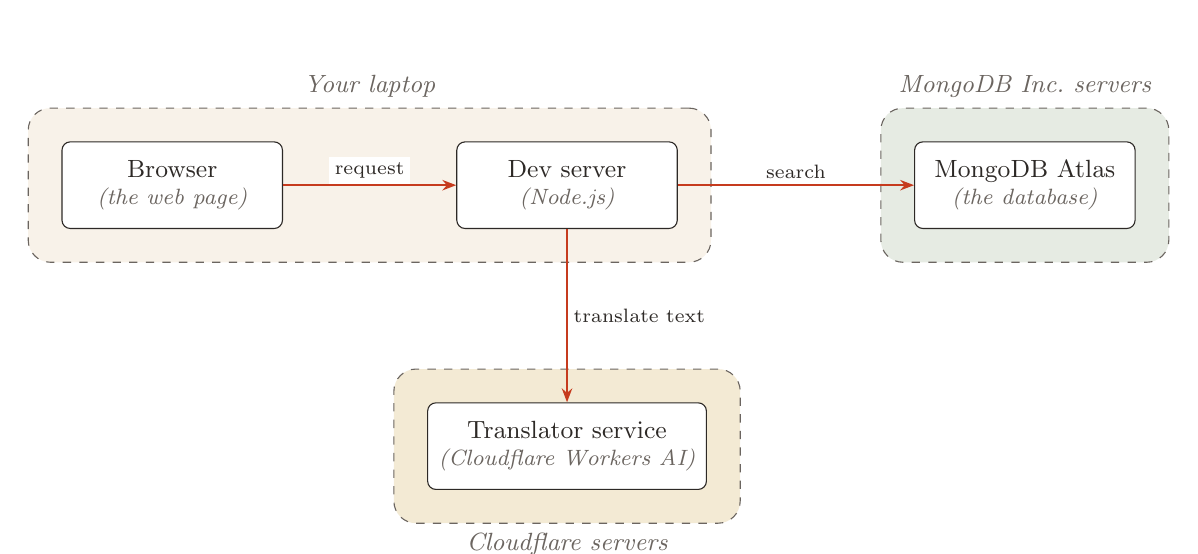
\begin{tikzpicture}[
  every node/.style={font=\small, text=charcoal},
  component/.style={
    draw=charcoal,
    rounded corners=3pt,
    minimum width=2.8cm,
    minimum height=1.1cm,
    fill=white,
    align=center,
    inner sep=4pt,
  },
  loclabel/.style={
    font=\small\itshape,
    text=mutedtext,
  },
  link/.style={
    -{Stealth[length=5pt]},
    thick,
    draw=usydred,
  },
  arrowlabel/.style={
    font=\scriptsize,
    text=charcoal,
    inner sep=2pt,
    fill=white,
  },
]
  \node[component] (browser) {Browser \\[-1pt] {\footnotesize\itshape\color{mutedtext}(the web page)}};
  \node[component, right=2.2cm of browser] (server) {Dev server \\[-1pt] {\footnotesize\itshape\color{mutedtext}(Node.js)}};
  \node[component, right=3.0cm of server] (atlas) {MongoDB Atlas \\[-1pt] {\footnotesize\itshape\color{mutedtext}(the database)}};
  \node[component, below=2.2cm of server] (cf) {Translator service \\[-1pt] {\footnotesize\itshape\color{mutedtext}(Cloudflare Workers AI)}};

  \begin{scope}[on background layer]
    \node[draw=mutedtext, dashed, rounded corners=8pt, inner sep=12pt,
          fill=sandstone!30,
          fit=(browser) (server),
          label={[loclabel]above:Your laptop}] {};
    \node[draw=mutedtext, dashed, rounded corners=8pt, inner sep=12pt,
          fill=eucalypt!15,
          fit=(atlas),
          label={[loclabel]above:MongoDB Inc.\ servers}] {};
    \node[draw=mutedtext, dashed, rounded corners=8pt, inner sep=12pt,
          fill=ochre!20,
          fit=(cf),
          label={[loclabel]below:Cloudflare servers}] {};
  \end{scope}

  \draw[link] (browser) -- node[arrowlabel, above]{request} (server);
  \draw[link] (server) -- node[arrowlabel, above]{search} (atlas);
  \draw[link] (server) -- node[arrowlabel, right]{translate text} (cf);
\end{tikzpicture}
\end{center}

\smallskip
\noindent{\small\itshape\color{mutedtext} The four pieces, grouped by where they actually run. The browser only ever talks to the dev server; the dev server is the only piece that talks to Atlas or Cloudflare.}

\medskip

\begin{enumerate}[leftmargin=2em,itemsep=8pt]
  \item \textbf{The web page (the browser).} What the researcher actually sees: a search box, a list of result cards, a couple of buttons to switch between user roles. It runs in any web browser. When the researcher types a query and presses Enter, the page sends a small request to the next piece.

  \item \textbf{The mini-server on your laptop (the ``dev server'').} A small program that listens for the requests coming from the web page and decides what to do with each one. It is the conductor of the system: it works out who is asking, asks the translator service to convert the query into numbers, asks the database to do the search, and sends the results back to the page. For now it runs on your laptop; in a production deployment it would run on a cloud server instead.

  \item \textbf{The database in the cloud (MongoDB Atlas).} A managed database, living on MongoDB's servers, that we access through their free tier. It stores every project record and answers search queries. The mini-server talks to it over the internet. One thing worth being explicit about: Atlas does only \emph{store and search} for us. It does not run any of our code, does not understand English, and does not check who is asking. Everything else happens in the mini-server.

  \item \textbf{The translator service (Cloudflare Workers AI).} A small service we rent from Cloudflare that takes a piece of text (for example, \emph{skin proteomics}) and returns a list of 1024 numbers. Why 1024 numbers? That is the topic of section 3. The mini-server calls this service once per search. We use Cloudflare's ``Workers AI'' offering because it is cheap, fast, and we already have an account.
\end{enumerate}

That is the entire system. The next section explains the one idea that ties it all together: how a list of 1024 numbers can stand in for the meaning of a sentence.

\section{The trick that makes it work}

The system needs to match what a researcher \emph{means} with what a past project is \emph{about}, even when the words don't line up. A query for \emph{skin proteomics} should find a project filed under \emph{dermatology, mass spectrometry}, because those phrases describe the same kind of work in different vocabulary. Plain keyword search cannot do this: the word \emph{skin} doesn't appear in the second project, so it would simply be missed.

The way around this is something called an \emph{embedding}.

\medskip

Imagine every short piece of text (a search query, a project summary, a paragraph from a paper) gets pinned as a single dot on a giant map. The map is not the usual two-directional kind: it has 1024 different directions. Where does each piece of text get pinned? That is decided by the translator service from section 2, which has been trained on enormous amounts of English text. The training has one extraordinarily useful side-effect: pieces of text with \emph{similar meanings} get pinned in \emph{nearby places} on the map.

So, on our map:

\begin{itemize}[leftmargin=2em,itemsep=2pt]
  \item \emph{Skin proteomics} lands somewhere.
  \item \emph{Dermatology, mass spectrometry} lands very close by, because the translator knows those phrases mean roughly the same thing.
  \item \emph{Mouse models of obesity} lands somewhere far away.
\end{itemize}

Each pin is, technically, just a list of 1024 numbers: its coordinates on the map. That list of numbers is what people mean when they say \emph{embedding} or \emph{vector}. Every time you see those words in the rest of this document, you can picture a pin on the map.

\subsection{How the system uses the map}

For each project, we send its summary text to the translator service \emph{once}, when it is first loaded into the database. The translator returns the 1024 numbers, and we save them with the project. From then on, every project in the database has its pin already pinned.

When a researcher types a query, the same translator service is called on the query text, giving \emph{its} pin. The database is then asked one question: \emph{of all the project pins, which 50 are closest to this query pin?} The answers, ordered by closeness, are the search results.

That is the whole idea behind the search. There is no other AI involved.

\section{A single query, step by step}

This section traces what happens when a researcher, logged in as an HDR student, types \emph{skin proteomics} into the search box and presses Enter. There are six steps. Three of the four pieces from section 2 do work along the way; the database does the heaviest lifting.

\begin{enumerate}[leftmargin=2em,itemsep=8pt]
  \item \textbf{The browser sends the query.} The web page bundles the query text, the user's role, and any chosen filters into a small request and sends it to the mini-server on your laptop.

  \item \textbf{The mini-server works out who is asking.} It reads the user's identity from the request. In the demo this comes from a simple header that says ``I am the HDR-student demo user''. In a real deployment, this step would check a login token from a single sign-on system instead.

  \item \textbf{The mini-server gets the query's pin.} It sends the text \emph{skin proteomics} to the translator service. Back comes a list of 1024 numbers: the query's pin on the map from section 3.

  \item \textbf{The mini-server asks the database to do the search.} It sends Atlas one instruction that combines two things: \emph{find the project pins closest to this query pin}, and \emph{leave out any project this user is not allowed to see}. In the actual code this is roughly:
  \begin{lstlisting}
[
  { $vectorSearch: {
      queryVector: [...1024 numbers...],
      filter: { /* "this user is allowed to see it" */ },
      limit: 50
  }}
]
  \end{lstlisting}
  Atlas runs both parts together and returns the matching projects, ordered by closeness. The access check happens \emph{inside} the database, before any data leaves it. Section 5 explains why that matters.

  \item \textbf{The mini-server quietly logs the query.} It writes a short record (the query text, the user, the number of results, the time) to a separate collection. This happens in the background and does not slow the response down. Over time, these logs become the data we use to improve the search.

  \item \textbf{The browser draws the results.} The mini-server sends the matching projects back to the web page, which renders them as cards. The researcher sees the projects most similar in meaning to \emph{skin proteomics}, with anything they are not allowed to see already filtered out.
\end{enumerate}

That is the whole journey. The next section zooms in on step 4, because the access-control behaviour there is what makes this version of the system meaningfully different from the simpler alternative.

\section{Who can see what}

Every project record in the database carries its own \emph{access list}: a small structure that declares who is allowed to see it. The structure has two parts.

\begin{lstlisting}
"access": {
  "preset":  "public",         // public | tier | restricted
  "viewers": ["tier:analyst", "tier:hdr", "user:elijah"]
}
\end{lstlisting}

The \texttt{preset} is a label for the rough sensitivity of the project: \texttt{public} (anyone can see it), \texttt{tier} (anyone in a particular role tier can see it), or \texttt{restricted} (only specifically named people). The \texttt{viewers} list spells out the actual identities allowed in. An identity can be a tier (\texttt{tier:hdr}, \texttt{tier:analyst}), a role (\texttt{role:supervisor}), or an individual person (\texttt{user:elijah}).

\subsection{The access check}

When the mini-server sends the search instruction in step 4, it adds a small extra clause that says, in effect, \emph{either the project is public, or the user shares an identity with someone on the viewers list}. In MongoDB syntax:

\begin{lstlisting}
{ $or: [
  { "access.preset":  "public" },
  { "access.viewers": { $in: ["user:demo-hdr", "tier:hdr"] } }
] }
\end{lstlisting}

This clause becomes part of the same database instruction that performs the search. Atlas applies it \emph{while} it does the search, not after. Projects this user cannot see never leave the database.

\subsection{Why this matters}

In the simpler alternative, all project metadata is shipped to the browser as one big file. The web page hides the projects this user is not allowed to see, but the data is already there: a researcher who knows where to look can open the page's network tab and read every project. ``Access control'' in that version is closer to a curtain than a lock.

In this version, restricted projects never leave the database in the first place. The decision happens inside Atlas, in the same step as the search itself. There is no window in which the application has data that the user is not authorised to read. That is what people mean when they say \emph{document-level} access control.

\subsection{The three demo users}

To make all of this visible in the demo, the mini-server pretends to support three different users. The role switcher in the UI maps the chosen role to one of these:

\begin{itemize}[leftmargin=2em,itemsep=2pt]
  \item \texttt{analyst}: a DASH analyst. Sees all 10 projects.
  \item \texttt{hdr}: an HDR student. Sees public projects and any project shared with the HDR-student tier (5 projects).
  \item \texttt{external}: an unaffiliated researcher. Sees public projects only (2 projects).
\end{itemize}

Switch between them in the UI, run the same search, and the result list visibly shrinks or grows. The exact same query is being run against the exact same database; only the user's identity changes.

\section{Running it tomorrow}

The system is already set up. After a laptop reboot, the only thing you need to do is start the mini-server. From a terminal:

\begin{lstlisting}
cd option_b
set -a; source .env; set +a
npm run dev
\end{lstlisting}

The first command moves into the project folder. The second loads the database connection string and other secrets from the \texttt{.env} file into the shell. The third starts the mini-server, which prints a URL (something like \texttt{http://localhost:8787}) once it is ready. Open that URL in a browser and the system is running.

If you ever change the project data and need to push the new versions into Atlas, the relevant commands (\texttt{npm run embed}, \texttt{npm run seed-acls}, \texttt{npm run ingest}) are documented in the setup notes. You do not need them for normal use.

\bigskip

\noindent\textcolor{usydred}{\rule{\textwidth}{1pt}}

\noindent\textit{\small See also: the setup notes (full setup steps), the access-control walkthrough, and the architecture tradeoffs note (why we chose this architecture over the simpler alternative).}

\end{document}
